\documentclass{article}

\textwidth=6.5in
\textheight=8.5in
\voffset=-54pt
\oddsidemargin=0in
\evensidemargin=0in
\setlength{\parskip}{8pt}
\setlength{\parindent}{0pt}

\usepackage{workbook}

\usepackage{handout}

\usepackage{exam}

\newcommand{\answerbox}[3][]{
    \fbox{\begin{minipage}[t][#2][c]{#3}
        #1
    \end{minipage}}
    }

\begin{document} 
 
{\large \mbox{} \hfill \bf Name:\underline{\hspace{3in}}}\\[2pt]
{\mbox{} \hfill \it (Please write your name neatly in print.)}\\[12pt]
{\large \mbox{} \hfill \bf HUID:\underline{\hspace{3in}}}
 
\medskip
 
\noindent
{\large\bf
Exam 2 Practice 1\\
Math Mb Spring 2025}
\noindent


{\Large
\begin{center}\textbf{Directions---Please read carefully!} \end{center}}

This is a practice test. The same directions will appear on the actual exam, so read them carefully.

\hrulefill 


This exam is subject to the Harvard College Honor Code. No calculators or any other aids are permitted.  Please write as neatly as possible, as answers that can't be read can't be graded and thus can't receive credit. To receive full credit, you must show relevant working
and include units when appropriate. 

You have 120 minutes to complete this exam. 

You may ask for scratch paper if you need additional space to write, but it will not be scanned or graded. Make sure to include all relevant working in this exam booklet in the space provided for each question.

\begin{center}\textbf{Good luck!}\end{center}


\vfill

\centering{
\emph{As a member of Harvard College, I pledge that I will not give or receive assistance on this exam.}}
\vspace{0.3in}

{\large \mbox{} \hfill \bf Signature:\underline{\hspace{3in}}}
\thispagestyle{empty}

\newpage


\begin{grading}
This p-set should be graded on completion on a 2-point scale as follows:

\begin{itemize}
\item 2 points: student made a serious attempt to solve the problems
\item 1 point: student made little attempt to solve the problems, and much of it is blank or missing
\item 0 points: assignment is missing or blank
\end{itemize}
\end{grading}




\begin{enumerate}
%% Definite integral.  Use as many or as a few as necessary.

\item The function $f(t)$ has domain $[0,7]$. The graph of the function $f(t)$ is given below. 
\begin{center} 
   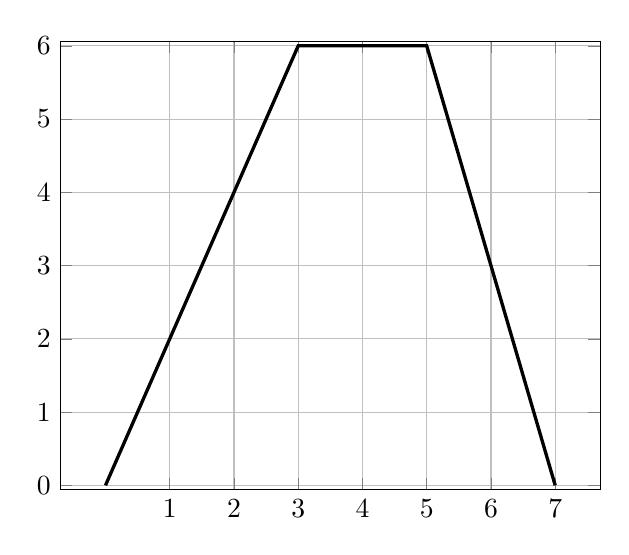
\begin{tikzpicture}
      \begin{axis}[cycle list=black, xtick={1, 2, ..., 12}, ytick={0,1,2,3,4,5,6}, grid=both, clip=false, enlarge y limits=0.01, axis
        line style={shorten >=-8pt}, xlabel style={xshift=8pt}, ylabel
        style={yshift=8pt}] %
        \addplot+[sharp plot, very thick] coordinates { (0, 0) (3, 6) (5,
          6) (7, 0) }node[right] {} ; %
    %
      \end{axis}
    \end{tikzpicture}
\end{center} 
    
\begin{enumerate} 
\item Let $A(x)=\displaystyle\int_3^x f(t)\,dt$. What is the value of $A(7)$?
\probonly{\vspace{0.25in}}

\begin{solution}
Starting at $x=3$, we see a rectangle with area 12 and a triangle with area 6. Thus $A(7)=12+6=18$.
\end{solution}

\item When is $A(x)$ increasing? Explain your reasoning.
\probonly{\vspace{1 in}}

\begin{solution}
By the fundamental theorem of calculus part 1, we know that $A'(x)=f(x)$. Thus the area function will be increasing whenever $f(x)$ is positive, and from the graph we see that $f(x)$ is positive for $0< x< 7$. We see that the area function will be increasing between $x=0$ and $x=7$.
\end{solution}


\item Calculate $\displaystyle \lim_{h \rightarrow 0} \frac{A(4+h)- A(4)}{h}$
\probonly{\vspace{0.5in}}

\begin{solution}
By the fundamental theorem of calculus part 1, we know that $A'(x)=f(x)$. The given limit is exactly the limit definition of the derivative of the area function at $x=4$. Thus we have $\displaystyle \lim_{h \rightarrow 0} \frac{A(4+h)- A(4)}{h} = A(4)=f(4)=6$.
\end{solution}

\item Let $B(x)=\displaystyle\int_2^x f(t)\,dt$. Simplify $B(x) - A(x)$ as much as possible.  Explain your reasoning.  Give a numerical answer if possible. 
\probonly{\vspace{1 in}}

\begin{solution}
Using the properties of the area function and integrals we get $$B(x) - A(x)= \int_2^x f(t) dt- \int_3^x f(t)dt=\int_2^3 f(t)dt=5$$
\end{solution}

\item Is $A(2)$ positive? Explain your reasoning. 

\begin{solution}
Using the properties of integrals and the previous part we get:

$A(2)=\displaystyle \int_3^2 f(t) dt = -\int_2^3 f(t) dt =-5$, so  $A(2)$ is not positive.
\end{solution}

\end{enumerate} 



\probonly{\newpage}
\item Evaluate the following limits. If a limit does not exist because it is $\infty$ or $-\infty$, indicate this as well.  If you are citing l'H\^opital's Rule at any point, be sure to indicate where and why it is valid to do so.

\begin{enumerate}
\item $\displaystyle \lim_{x\to 0} \frac{\arctan x}{x}$

\begin{solution}
Plugging in $x=0$, we verify that we have a $\frac{0}{0}$ indeterminate form, and hence we can use l'H\^opital's Rule. Applying l'H\^opital's Rule, we get $$\lim_{x\to 0} \displaystyle\frac{\arctan x}{x}=\lim_{x\to0} \frac{\frac{1}{1+x^2}}{1}=1.$$
\end{solution}

\vfill 

\item $\displaystyle \lim_{x\to 1}\frac{\cos(\pi x) +x}{(x-1)(x+5)}$


\begin{solution}
Again plugging in $x=1$, we get $\frac{0}{0}$ indeterminate form, and hence we can use l'H\^opital's Rule. Applying l'H\^opital's Rule, we get $$\lim_{x\to 1}\frac{\cos(\pi x) +x}{(x-1)(x+5)}=\lim_{x\to 1}\frac{-\pi \sin(\pi x) +1}{(x-1)+(x+5)}=\frac{1}{6}.$$
\end{solution}


%\item $\displaystyle \lim_{x\to \infty}\frac{e^x}{x^{10,000,000}}$

\vfill

\item $\displaystyle \lim_{x\to \infty} \frac{(1.999)^x + x^2 + 4\sqrt{x}}{1+ x^{\frac14}+\ln x +(1.5)^x}$

\begin{solution}
In this problem we examine the relative growth rates. Notice that the fastest growing term in the numerator is $(1.999)^x$, and the fastest growing term in the denominator is $(1.5)^x$. As $(1.999)^x$ grows much more quickly than $(1.5)^x$, we get $\displaystyle \lim_{x\to \infty} \frac{(1.999)^x + x^2 + 4\sqrt{x}}{1+ x^{\frac14}+\ln x +(1.5)^x}=\infty$
\end{solution}

\vfill

\end{enumerate}

%\newpage
%\item Sketch the graph of $f(x)=\sqrt{x} \ln (x)$ by first working through the following parts.

%\begin{enumerate}
%\item Find the domain of $f(x).$\vspace{0.2in}

%\begin{solution} 
%The function $f(x)$ is the product of two functions we know well, $\sqrt{x}$ and $\ln(x)$. The domain of $f(x)$ will then be all numbers that can be plugged into both of these functions;  the domain is $x>0$.

%\end{solution} 
%\item Find the $x$ and $y$ intercepts, if any.

%\begin{solution} 
%There are no $y-$intercepts since $x=0$ is not in the domain of the function. To find any $x-$intercepts we need to solve the equation $\sqrt{x} \ln(x) =0$. This is true only when $\ln(x) = 0$. That means that $x=1$ is the only $x-$intercept.
%\end{solution} 

%\vfill
%\item $\displaystyle \lim_{x\to \infty}\sqrt{x} \ln (x)$\vspace{0.1in} 

%\begin{solution} 
%Both $\ln(x)$ and $\sqrt{x}$ increase without bound as $ x \rightarrow \infty$, so 

%$$ \displaystyle \lim_{x\to \infty}\sqrt{x} \ln (x) = \infty$$ 


%\end{solution} 
%\item $\displaystyle \lim_{x\to 0^{+}}\sqrt{x} \ln (x)$
%\begin{solution} 
%Notice that this is an indeterminate limit of the form $0 \cdot - \infty$. In order to use L'Hopital's rule we need to transform it into a $\frac{0}{0}$ or $\frac{ \infty}{\infty}$. 

%\begin{align*}
%\lim_{x\to 0^{+}}\sqrt{x} \ln (x) &= \lim_{x\to 0^{+}} \frac{\ln(x) } {\frac{1}{x}}\\ 
%&= \lim_{x\to 0^{+}} \frac{ \frac{1}{x}} {-\frac{1}{x^2}}\\
%&= \lim_{x\to 0^{+}} -x\\
%&=0
%\end{align*} 

%\end{solution} 

%\vfill\vfill
%\item Find where $f(x)$ is increasing and decreasing.\vspace{1.5in}

%\begin{solution} 
%We can use the derivative to find where the function is increasing and where it is decreasing. The function is increasing when $f'(x)>0$ and the function is decreasing when $f'(x) <0$. 

%$$f'(x) = \sqrt{x} \frac{1}{x} + \frac{1}{2} x^{-\frac{1}{2}} \ln(x) $$ 

%To find where $f'(x)>0$ and where $f'(x) <0$. We want to find where $f'(x) = 0$. 

%\begin{align*} 
%f'(x) & =0 \\ 
%\sqrt{x} \frac{1}{x} + \frac{1}{2} x^{-\frac{1}{2}} \ln(x)  & = 0 \\
%x^{-\frac{1}{2}}  + \frac{1}{2} x^{-\frac{1}{2}} \ln(x) & = 0\\ 
%x^{-\frac{1}{2}}( 1 +\frac{1}{2} \ln(x) )& = 0 \\
%1 + \frac{1}{2} \ln(x) & = 0 \\ 
%x = e^{-2 }
%\end{align*} 

%On the interval $(0, \frac{1}{e^{-2}}) $, $f'(x) <0$ and so $f(x)$ is decreasing on that interval. \\
%On the interval $( \frac{1}{e^{-2}}, \infty)$, $f'(x) >0$ and so $f(x)$ is increasing on that interval. 


%\end{solution} 
%\item Given that $\displaystyle f''(x)=\frac{-\ln x}{4x^{3/2}},$ find where $f(x)$ is concave up and concave down.

%\begin{solution} 
%The second derivative is helpful because when $f''(x)>0$ the function is concave up and when $f''(x) <0$ the function is concave down. We see that $f''(x)$ only has one zero at $x=1$. For values in the interval $(0, 1)$, $f''(x) >0$ and for values in the interval $(1, \infty)$, $f''(x)< 0$. 
%\end{solution} 

%\vspace{.6in}

%\item Accounting for the previous parts, sketch the graph of $f(x)$ below.  Label your intercept(s) and extrema.  Clearly indicate changes in concavity.

%\begin{center} \problemonly{
%\begin{tikzpicture}[scale=1.2,y=0.75 cm]
    %\draw[step=1, loosely dotted] (-3,-3) grid (3,3);
    %\path[use as bounding box] (-2,-1) rectangle (5,5);
 %   \draw[->] (-3.2,0) -- (3.25,0) node[right] {$x$};
  %  \draw[->] (0,-3.25) -- (0,3.25) node[above] {$y$};
   % \foreach \x/\xtext in {-3/-3,-2/-2,-1/-1,1/1, 2/2, 3/3}
   % \draw[shift={(\x,0)}] (0pt,2pt) -- (0pt,-2pt) node[below] {$\xtext$};
   % \foreach \y/\ytext in {-3/-3,-2/-2,-1/-1,1/1, 2/2, 3/3}
   % \draw[shift={(0,\y)}] (2pt,0pt) -- (-2pt,0pt) node[left] {$\ytext$};

%\end{tikzpicture}}
%\end{center} 
%\begin{solution} 
%\begin{tikzpicture}[scale=1.2,y=0.75 cm]

%     \draw[domain=0.0001:5,smooth,variable=\x,blue] plot ({\x},{ln(\x)*\x^.5 });
    %\draw[step=1, loosely dotted] (-3,-3) grid (3,3);
    %\path[use as bounding box] (-2,-1) rectangle (5,5);
 %   \draw[->] (-3.2,0) -- (3.25,0) node[right] {$x$};
  %  \draw[->] (0,-3.25) -- (0,3.25) node[above] {$y$};
%    \foreach \x/\xtext in {-3/-3,-2/-2,-1/-1,1/1, 2/2, 3/3}
 %   \draw[shift={(\x,0)}] (0pt,2pt) -- (0pt,-2pt) node[below] {$\xtext$};
 %   \foreach \y/\ytext in {-3/-3,-2/-2,-1/-1,1/1, 2/2, 3/3}
 %   \draw[shift={(0,\y)}] (2pt,0pt) -- (-2pt,0pt) node[left] {$\ytext$};

%\end{tikzpicture}

%\end{solution} 

%\end{enumerate}

\begin{comment} 
Save this for the final!
\item Let $$g(x)=\int_2^{x^3-3x^2}{e^{\sin{t}}dt}.$$

\begin{enumerate}
    \item  Compute $g'(x)$.

\vfill

\item Find and classify critical points of $g$.

\vfill

\item Find intervals where $g$ is increasing/decreasing.

\vfill

%\item Compute $g''(x)$.
\end{enumerate}
%\newpage
%\item %% This is my R_n L_n question -- will be added before the meeting!
\newpage
\end{comment}

\newpage

\item \label{spring2012-mb-midterm2-area-function}



  In this problem, you'll look at $ A(x) = \displaystyle \int_{3}^x
  f(t)\,dt$, where $f$ is the function whose graph is given below.

  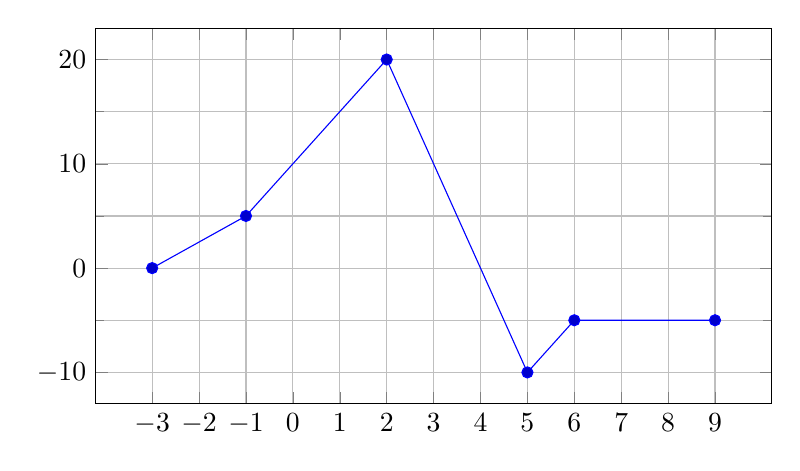
\begin{tikzpicture}
    \begin{axis}[grid=major, xtick={-3, -2, ..., 9}, ytick={-10, 0, 10,
        20}, minor ytick={-15, -5, ..., 25}, grid=both, width=4in,
      height=2.5in] 
      \addplot+[sharp plot] coordinates { (-3, 0) (-1, 5) (2, 20) (5, -10)
        (6, -5) (9, -5) }; 
    \end{axis}
  \end{tikzpicture}

  \begin{enumerate}
  \item \label{spring2012-mb-midterm2-area-function-evaluate}

    \begin{problem}[\vfill]
      Evaluate $ A(2)$.
    \end{problem}    

    \begin{solution}
      This is $\displaystyle \int_{3}^2 f(t)\,dt$, which equals
      $\displaystyle -\int_{2}^3 f(t)\,dt$. $\displaystyle \int_{2}^3
      f(t)\,dt$ is the area under the curve between $x=2$ and $x=3$.  This
      forms a trapezoid, and we can compute its area as 15.  Thus, the
      answer is $\boxed{-15}$.
    \end{solution}

  \item

    \begin{problem}[\vfill]
      Find \textbf{two} different $x$-intercepts of $A(x)$. 
    \end{problem}

    \begin{solution}
      We are looking for values of $x$ where $A(x) = 0$, i.e., where
      $\displaystyle \int_3^x f(t)\,dt = 0$.  One such value is $x =
      \boxed{3}$, since $\displaystyle \int_3^x f(t)\,dt$.  Another such
      value is $x = \boxed{5}$ because $\displaystyle \int_3^5 f(t)\,dt =
      0$.
    \end{solution}

  \item \label{spring2012-mb-midterm2-area-function-c}
    \begin{problem}[\vfill]
      For what values of $x$ in $(-3, 9)$ is $ A(x)$ decreasing? 
    \end{problem}

    \begin{solution}
      Our usual strategy for such a question is to make a sign chart for
      $ A'$.  By FTOC 1, $ A'(x) = f(x)$.  So, we really want
      to make a sign chart for $f$:
      \begin{center}
        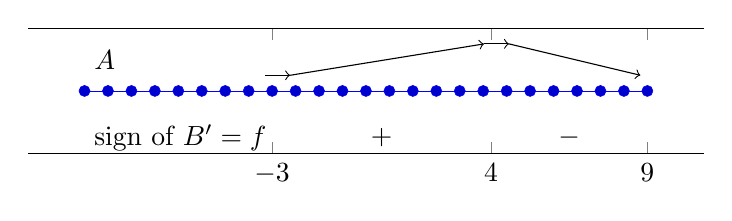
\begin{tikzpicture}
          \begin{axis}[axis y line=none, x axis line style={-}, xtick={-3., 4., 9.}, xticklabels={$-3$, $4$, $9$}, ymin=-2, ymax=2, height=1.25in, width=4in]
            \addplot+[domain=-9.:9., very thin]{0};
            \draw (axis cs: -9., -1.5) node[right] {sign of $B' = f$};
            \draw (axis cs: -9., 1) node[right] {$ A$};
            \draw (axis cs: 0.5, -1.5) node{$+$};
            \draw[->, xshift=2pt] (axis cs: -3.4, 0.5) -- (axis cs: -2.6, 0.5);
            \draw[->, xshift=2pt] (axis cs: -2.6, 0.5) -- (axis cs: 3.6, 1.5);
            \draw (axis cs: 6.5, -1.5) node{$-$};
            \draw[->, xshift=2pt] (axis cs: 4.4, 1.5) -- (axis cs: 8.6, 0.5);
            \draw[->, xshift=2pt] (axis cs: 3.6, 1.5) -- (axis cs: 4.4, 1.5);
          \end{axis}
        \end{tikzpicture}
      \end{center}
      So, $ A$ is decreasing on \fbox{$(4, 9)$}.
    \end{solution}

  \item
    \begin{problem}[\vfill\vfill]
      Does $ A(x)$ have an absolute maximum value on $[-3, 9]$?  If
      so, what is this value and where (that is, at what $x$-value) does
      it occur?  If not, explain why not.
    \end{problem}

    \begin{solution}
      From the sign chart we drew in
      (c), $A$ has its
      absolute maximum at $\boxed{x = 4}$.
    \end{solution}

  \item % added
    \label{spring2012-mb-midterm2-area-function-abs-min}
    \begin{problem}[\vfill\vfill\newpage]
      Does $ A(x)$ have an absolute minimum value on $[-3, 9]$?  If
      so, 
      where (that is, at what $x$-value) does it occur?  If not, explain
      why not.
    \end{problem}

    \begin{solution}
      Since $[-3, 9]$ is a closed interval and $A$ is continuous,
      $A$ must have an absolute minimum on $[-3, 9]$.  From the
      sign chart we drew in (c),
      the absolute minimum is either at $x = -3$ or $x = 9$.  To decide
      between these two, we can plug both into $A$ to see which
      gives the lower value:
      \begin{align*}
        A(-3) &= \int_{3}^{-3} f(t)\,dt = - \int_{-3}^3 f(t)\,dt \\
        A(9) &= \int_3^9 f(t)\,dt
      \end{align*}
      Just by comparing these visually, we can see that $ A(-3)$ is
      more negative, so the absolute minimum is at $\boxed{x = -3}$. 
    \end{solution}

  \item
    \begin{problem}[1.25in]
      For what values of $x$ in $(-3, 9)$ is $ A(x)$ concave down?
    \end{problem}

    \begin{solution}
      $A$ is concave down when $A' = f$ is decreasing, which
      happens on $\boxed{(2, 5)}$.
    \end{solution}

  \item \label{spring2012-mb-midterm2-area-function-sketch}
    \begin{problem}[\newpage]
      On the axes below, sketch a rough graph of $ A(x)$ on $[-3,
      9]$.  

      (\emph{Note:} Your graph need not be completely accurate, but it
      should accurately portray the concavity of $A(x)$ and
      everything else you have found in this problem.)

      \probonly{
      \begin{tikzpicture}
          \begin{axis}[xtick={-3, -2, ..., 9}, 
          xmin=-3, xmax=9.5, width=4in, ytick=\empty]
              \addplot[draw=none]{x};
          \end{axis}
      \end{tikzpicture}}
    \end{problem}

    \begin{solution}
      \begin{center}
        \begin{tikzpicture}
          \begin{axis}[cycle list=black, xtick={-3, -2, ..., 9},
            width=4in, height=2.5in, xmin=-3, xmax=9.5, ytick={-15}]
            \addplot+[domain=6.:9.]{22.5 - 5.*x};
            \addplot+[domain=5.:6.]{2.5*(45. - 14.*x + x^2)};
            \addplot+[domain=2.:5.]{-5.*(15. - 8.*x + x^2)};
            \addplot+[domain=-1.:2.]{2.5*(-18. + 4.*x + x^2)};
            \addplot+[domain=-3.:-1.]{1.25*(-37. + 6.*x + x^2)};
          \end{axis}
        \end{tikzpicture}
      \end{center}


      The key features your graph should have are:
      \begin{itemize}
      \item It has $x$-intercepts at $x = 3$ and $x = 5$.
      \item It increases on $(-3, 4)$ and decreases on $(4, 9)$.
      \item It's concave up on $(-3, 2)$, concave down on $(2, 5)$,
        concave up on $(5, 6)$, and linear (with slope $-5$) on $(6, 9)$. 
      \end{itemize}
      We also know that the graph includes the point $(2, -15)$. 
    \end{solution}

  \end{enumerate}
  \vfill
\item R2 the robot is leaking coolant at an alarming rate!  

The leak began at midnight, and is growing steadily worse.  Data on the rate at which coolant is leaking out is provided in the table below.

   \begin{tabular}{c | c}
   \hline
   Time (in hours past midnight) & Rate of coolant leak (in $\textrm{L}/\textrm{hr}$) \\
   \hline
   0 & 1.8 \\
   0.5 & 2.4 \\
   1.0 & 2.8 \\
   1.5 & 3.0 \\
   2.0 & 3.2 \\
  \hline
   \end{tabular}

   \begin{enumerate}

   \item  Use a left-hand sum with $4$ rectangles to estimate the amount of coolant R2 has lost between midnight and $2$ am.  
   
\begin{solution}
The left-hand sum approximation is given by $L_4=\frac12(1.8+2.4+2.8+3)=5$ L.
\end{solution}
    \vfill
   \item  Use a right-hand sum with $4$ rectangles to estimate the amount of coolant R2 has lost between midnight and $2$ am. 
   
\begin{solution}  The right-hand sum approximation is given by $R_4=\frac12(2.4+2.8+3+3.2)=5.7$ L.
\end{solution} 
   \vfill
   
   \item R2's warning system will go off if his coolant level drops below $2\ \text{L}$.  At midnight he had $8\ \text{L}$ of coolant.  Has his warning system sounded by $2$ am? Explain.
   
\begin{solution}
No, he lost at most 5.7 L and this is an over estimate.
\end{solution} 
   \vfill

  \item From $2$ am onwards, R2 loses coolant at a constant rate of $3.2\ \text{L}/\text{hr}$.  R2's friend Luke is bringing R2 more coolant.  If Luke arrives at $3$ am, will he get there before R2 runs out of coolant?
  
\begin{solution}   From the underestimate, R2 will lose $5$ L and then another 3.2 L between 2-3 am.  This means that he will lose at least 8.2 L, (and possibly more).  He will certainly run out of coolant by 3 am.\end{solution} 
  \vfill

  \end{enumerate}

\probonly{\newpage}


\item 

  A  panda bear and a raccoon  are running a race against each other.  The
  panda's velocity $p(t)$ and the raccoon's velocity $r(t)$ are both shown
  below in feet per second. The race begins at the starting line at time $t=0$. 

  \begin{center}
    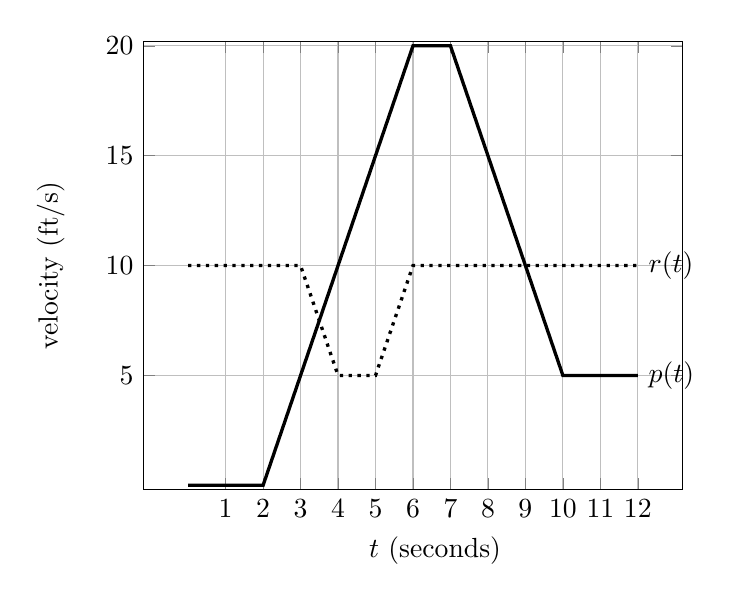
\begin{tikzpicture}
      \begin{axis}[cycle list=black, xtick={1, 2, ..., 12}, ytick={5, 10,
          ..., 30}, grid=both, clip=false, enlarge y limits=0.01, axis
        line style={shorten >=-8pt}, xlabel style={xshift=8pt}, ylabel
        style={yshift=8pt}, xlabel={$t$ (seconds)}, ylabel={velocity
          (ft/s)}] %
        \addplot+[sharp plot, very thick] coordinates { (0, 0) (2, 0) (6,
          20) (7, 20) (10, 5) (12, 5) } node[right] {$p(t)$} ; %
        \addplot+[sharp plot, very thick, dotted] coordinates { (0, 10)
          (3, 10) (4, 5) (5, 5) (6, 10) (12, 10) } node[right] {$r(t)$}
        ; %
      \end{axis}
    \end{tikzpicture}
  \end{center}

  \begin{enumerate}  
  
  \item The panda is taking a short break at $t = 0$.  How can you tell this from the graph?\vfill
  \begin{solution} 
  The graph given is the velocity for the two animals. We see that the velocity for the Panda is $0$ for the first $2$ seconds. 
  
  \end{solution} 
  \item Let $L$ be the raccoon's lead when the panda first starts moving
      again.  Write an expression for $L$ involving a definite integral.\vfill
  
  
  \begin{solution} 
  $$ L = \int_0^2 r(t) dt$$ 
  \end{solution} 
  
  \item Calculate $L$ exactly and include units.\vfill
  
  \begin{solution} 
For the first two seconds the speed of the raccoon is constant, this means definite integral can be calculated by finding the volume of a rectangle. The rectangle has height $10$ and base $2$. So $L = 20 $ ft
  \end{solution} 
  
   

  \item  Let $M$ be the distance between the raccoon and the panda at
      time $t=4$.  Write an expression using a definite integral for $M$. 
      
      \probonly{\vfill}
   
\begin{solution}
  
     $$M = \int_{0}^4 r(t) - p(t)dt$$ 

  \end{solution}

  \item Calculate $M$ exactly. What are the units?%\vfill

\begin{solution} 
There are many ways to go about calculating $M$. The goal is to find the area between the curves $r(t)$ and $p(t)$ on the domain $[0,4]$. Our strategy is to use properties of the definite integral. 

$$\int_{0}^4 r(t) - p(t)dt = \int_{0}^4 r(t) dt- \int_{0}^4 p(t)dt$$


The integral $\int_{0}^4 r(t) dt$ can be calculated by computing the area of a rectangle plus the area of a trapezoid.  
$$ \int_{0}^4 r(t) dt = 20+17.5 = 37.5$$

The integral $\int_{0}^4 p(t) dt$ by computing the area of a triangle. 

$$\int_{0}^4 r(t) dt = 10$$

The distance between the panda and the raccoon is $37.5-10 = 27.5$ ft. 

\end{solution} 

\newpage

Problem 5 continued: The
  panda's velocity $p(t)$ and the raccoon's velocity $r(t)$ are both shown
  below in feet per second.   

  \begin{center}
    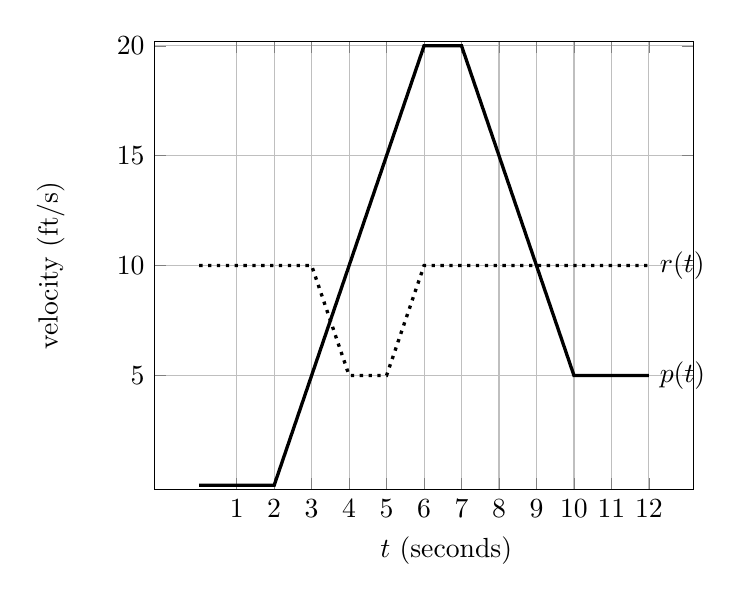
\begin{tikzpicture}
      \begin{axis}[cycle list=black, xtick={1, 2, ..., 12}, ytick={5, 10,
          ..., 30}, grid=both, clip=false, enlarge y limits=0.01, axis
        line style={shorten >=-8pt}, xlabel style={xshift=8pt}, ylabel
        style={yshift=12pt}, xlabel={$t$ (seconds)}, ylabel={velocity
          (ft/s)}] %
        \addplot+[sharp plot, very thick] coordinates { (0, 0) (2, 0) (6,
          20) (7, 20) (10, 5) (12, 5) } node[right] {$p(t)$} ; %
        \addplot+[sharp plot, very thick, dotted] coordinates { (0, 10)
          (3, 10) (4, 5) (5, 5) (6, 10) (12, 10) } node[right] {$r(t)$}
        ; %
      \end{axis}
    \end{tikzpicture}
  \end{center}
   
  \item What is the fastest speed the panda travels during the race?  What is the raccoon's fastest speed? \vfill
  \begin{solution} 
  The panda travels has a max speed of 20 ft/s. The raccoon travels at a max speed of 10 ft/s. 
  \end{solution} 
  
  \item  Who is ahead at time $t=12$? Please justify.\vfill
   
\begin{solution} 
The raccoon is ahead at $t=12$. You can tell since 

$$\int_{0}^{12} p(t) dt > \int_{0}^{12} r(t) dt$$

This calculation is probably done quickest by counting rectangles. The raccoon is not up by much at $t=12$.
\end{solution} 


  \item  When is the raccoon's lead on the panda increasing most rapidly?  At what rate is it increasing then?\vfill
    
\begin{solution} 
During the first two seconds $r(t) - p(t)$ obtains a global maximum. You can see this visually since the graph for $r(t)$ is 10 units above the graph for $p(t)$ in the first two seconds, which is the largest gap between the two graphs in which $r(t)$ is greater. 

During this time, the raccoon's velocity exceeds the panda's by 10 feet per second. Thus, the raccoon's lead increases by 10 feet per second. 

\end{solution} 

  \item When is the raccoon furthest ahead of the panda?

  \probonly{\vfill}
    
\begin{solution} 
The raccoon is furthest ahead at $t=3.5$. Notice that $r(t) - p(t)$ is the rate at which the distance between the two animals is changing. To maximize the distance between the two animals, we should find where the derivative is zero. That is when $r(t) = p(t)$. This happens at $t=3.5$ and $t=9$. You can see the point $t=3.5$ is a local max and $t=9$ is a local min. From the previous parts you know that at the end point $t=12$ the raccoon is not as far ahead as he is at time $t=3.5$. 

\end{solution} 
   

  %\item  After the start of the race, how many times do the raccoon and the panda pass each other?
  %After the start of the race, how many times are the panda and the raccoon at the same distance from the start at the same time?
   

    
  \end{enumerate}
   
   \probonly{\newpage}
   \item Let  $f(x)$ be a positive and increasing function where $\displaystyle\int_1^4 f(x)\ dx = 6$.  Give values for the expressions below, or say there is not enough information to do so. % If you need more information, what information do you need?
\begin{enumerate}
\item $6+\displaystyle\int_1^4f(x) \, dx$\vfill
\begin{solution} 
We know that $\displaystyle\int_1^4f(x) \, dx = 6$ and so the answer to this question is just $6 +6=12$. 

\end{solution} 
\item $\displaystyle\int_1^8 f(x) \, dx + \int_8^4 [f(x)+6] \, dx$\vfill
\begin{solution} 
We can use our integral properties to rewrite: 
$$\displaystyle\int_1^8 f(x) \, dx + \int_8^4 [f(x)+6] \, dx= \displaystyle\int_1^8 f(x) \, dx + \int_8^4 f(x)\, dx + \int_8^4 6 \, dx$$ 
$$= \displaystyle\int_1^8 f(x) \, dx - \int_4^8 f(x)\, dx - \int_4^8 6 \, dx $$
$$= \displaystyle\int_1^4 f(x) \, dx - \int_4^8 6 \, dx$$
$$ = 6 - 24 = -18$$ 


\end{solution} 

\item $\displaystyle\int_4^1 f(x+8)\, dx$

\begin{solution} 
We do not have enough information to solve this problem.

\end{solution} 

\vfill
%\item $\displaystyle\int_3^7 f(x+3)\, dx$\vfill
\item $\displaystyle\int_{-7}^{-4} f(x+8)\, dx$

\begin{solution} 
The function $f(x+8)$ is the same as the function $f(x)$ translated 8 units to the left. This means that 

$$ \displaystyle\int_{-7}^{-4} f(x+8)\, dx =\displaystyle\int_{1}^{4} f(x)\, dx =6  $$

\end{solution} 

\vfill

%\item $\displaystyle\int_{-2}^1 f(x+3)\, dx$\vfill

%\item $\displaystyle\int_1^4f(x) +6 \, dx$\vfill
\item $\displaystyle\int_1^4\left(|x-2| +f(x) - 6\right)\, dx$\vfill

\begin{solution} 

The most missed part of this question is identifying that we can compute $\displaystyle\int_1^4|x-2| \,dx$ geometrically. The area we need to compute can be broken up into two triangles. One triangle has area $\frac{1}{2}$ the other triangle has area $2$. This means the that entire integral we want to calculate is 

$$ 2.5 +6- 18= -9.5$$ 

\end{solution}

%\item $\displaystyle\int_1^4f(x) - 6\, dx$\vfill
\item $\displaystyle\int_0^4\left(f(x) + \sqrt{16-x^2}\right) \, dx +\int_1^0f(x)\, dx$\vfill
\begin{solution} 
We can use properties of integrals 

$$\displaystyle\int_0^4\left(f(x) + \sqrt{16-x^2}\right) \, dx +\int_1^0f(x)\, dx = \displaystyle\int_0^4\left(f(x) + \sqrt{16-x^2}\right) \, dx -\int_0^1f(x)\, dx$$

$$ = \displaystyle\int_1^4f(x)  \, dx +\int_0^4 \sqrt{16-x^2} \, dx$$

$$ = 6 + 4 \pi$$ 

\end{solution} 

\pspace{\newpage}



%\item $\displaystyle\int_1^4f(x) + x \, dx$\vfill
\item Let $R_5$ be the approximation of  $\displaystyle\int_1^4 f(x) \, dx$ by a right Riemann sum with 5 equal sub-intervals. Let $\Delta x$ be the width of the sub-intervals, and let $x_k$ be the $x$-value used for the $k$-th sub-interval.  

\begin{enumerate}
    \item 
    \begin{problem}
        Write down the value of $\Delta x$.
    \end{problem}
    \pspace{\vfill}

    \begin{solution}
        $\Delta x = \dfrac{4-1}{5}= \dfrac{3}{5}$
    \end{solution}

        \item 
    \begin{problem}
        Write down a formula for $x_k$ in terms of $k$.
    \end{problem}
    \pspace{\vfill}

    \begin{solution}
        $x_k = 1+k\Delta x = 1+ \frac{3}{5}k$
    \end{solution}

\item 
\begin{problem}
    Write down a formula for $R_5$ \textbf{using sigma notation. }
\end{problem}
\pspace{\vfill}

\begin{solution}
    $\displaystyle R_5 = \sum_{k=1}^5 \tfrac{3}{5}f(1+\tfrac{3}{5}k)$
\end{solution}

\end{enumerate}


% \item For $R_n,$ rewrite the limit in terms of $x_k$ and $\Delta x:$ %$\displaystyle\lim_{n\to \infty} R_n=\lim_{n\to \infty}\underline{\sum_{k=1}^nf(x_k)\Delta x} $
% Simplify the expression: $\displaystyle\lim_{n\to \infty} R_n= $
\item Put the following six expressions in increasing order. If
two expressions are equal, write an equals sign between them in the box. Otherwise, use the appropriate inequality symbol.

\hfill $\displaystyle\int_1^4 f(x)\, dx$ \hfill 
$\displaystyle\lim_{n\to \infty} R_n$ \hfill
$L_5$ \hfill
$R_5$ \hfill
$L_{100}$ \hfill
$R_{100}$ \hfill\strut

\probonly{
\hfill \uline{\hspace{0.6in}\vphantom{$\dfrac{0}{0}$}} \hfill \fbox{\phantom{$\leq$}} \hfill
\hfill \uline{\hspace{0.6in}\vphantom{$\dfrac{0}{0}$}} \hfill 
\fbox{\phantom{$\leq$}} \hfill
\hfill \uline{\hspace{0.6in}\vphantom{$\dfrac{0}{0}$}} \hfill 
\fbox{\phantom{$\leq$}} \hfill
\hfill \uline{\hspace{0.6in}\vphantom{$\dfrac{0}{0}$}} \hfill 
\fbox{\phantom{$\leq$}} \hfill
\hfill \uline{\hspace{0.6in}\vphantom{$\dfrac{0}{0}$}} \hfill 
\fbox{\phantom{$\leq$}} \hfill
\hfill \uline{\hspace{0.6in}\vphantom{$\dfrac{0}{0}$}} \hfill\null
}
\pspace{\vfill}


\begin{solution}
\begin{center}
 \underline{$L_5$}\    \fbox{{$<$}}\    \underline{ $L_{100}$}\    \fbox{{$<$}}\     \underline{$ \displaystyle\int_1^4 f(x)\, dx$}\    \fbox{$=$}\     \underline{$ \displaystyle\lim_{n\to \infty} R_n$}\    \fbox{$<$}\    \underline{$R_{100}$}\    \fbox{$<$}\     \underline{$R_5$} \end{center}
 \end{solution}
\end{enumerate}


\newpage

% \item %Matt's question 
% Write down the domain and range of the following functions:
%         \begin{enumerate}
%             \item $f(x) = \arctan(x)$ \hfill Domain: \hfill Range: \hfill \phantom{.}

%             \begin{solution}
%                 The domain of $f(x)= \arctan(x)$ is $(-\infty, \infty)$ (coming from the range of $\tan(x)$ and it's range is $\Big( -\dfrac{\pi}{2}, \dfrac{\pi}{2}\Big)$ coming from the restricted domain of $\tan(x)$.
%             \end{solution}
            
%             \vspace{.5 in}
            
%             \item $f(x) = \arcsin(x)$ \hfill Domain: \hfill Range: \hfill \phantom{.}

%             \begin{solution}
%                 The domain of $f(x)= \arcsin(x)$ is $[-1, 1]$ (coming from the range of $\sin(x)$) and it's range is $\Big[ -\dfrac{\pi}{2}, \dfrac{\pi}{2}\Big]$ coming from the restricted domain of $\sin(x)$.
%             \end{solution}
            
%             \vspace{.5 in}
%             \item $f(x) = \arccos(x)$ \hfill Domain: \hfill Range: \hfill \phantom{.}

%             \begin{solution}
%                 The domain of $f(x)= \arccos(x)$ is $[-1, 1]$ (coming from the range of $\cos(x)$) and it's range is $[0,\pi]$ coming from the restricted domain of $\cos(x)$.
%             \end{solution}
            
%             \vspace{.5 in}

%         \end{enumerate}

% \item You are driving north along a straight road. 
% To your right, there is an 30-foot-wide billboard. The left edge
% of the billboard is 
% 10 feet from the road. At what distance $x$ from the billboard
% is your viewing angle $\theta$ at a maximum?

% 
\includegraphics[scale=0.3]{Assessments/Midterms/billboard.png}

% \begin{solution}
% First, we need to express $\theta$, the quantity we want to maximize, in terms of $x$. We can express $\theta$ as
% $\theta = \alpha - \beta$, where $\alpha$ is the angle formed by the side of the road and the line of sight to the right side of the billboard and $\beta$ is the angle formed by the side of the road and the line of sight to the left side of the billboard.

% Using trigonometry, we know that 
% \[\tan(\alpha)=\dfrac{40}{x} \quad \text{and} \quad 
% \tan(\beta)=\dfrac{10}{x},\] 
% therefore 
% \[\alpha = \arctan\biggl(\dfrac{40}{x}\biggr) \quad \text{and} 
% \quad \beta = \arctan\biggl(\dfrac{10}{x}\biggr).\]

% This means that we can express $\theta$ as a function of $x$ 
% on the domain $x > 0$ as follows.
% \[\theta = \arctan\biggl(\dfrac{40}{x}\biggr) - 
% \arctan\biggl(\dfrac{10}{x}\biggr)\]

% To maximize this function, let's first find the critical points
% by finding the derivative.
% \begin{align*}
%     \dfrac{d\theta}{dx} &= \left(\dfrac{1}{1+(\frac{40}{x})^2}\right)
%     \left(-\dfrac{40}{x^2}\right) - \left(\dfrac{1}{1+(\frac{10}{x})^2}\right)
%     \left(-\dfrac{10}{x^2}\right) \\
%     \intertext{To help us solve for the critical points,
%     let's simplify the derivative.}
%     \dfrac{d\theta}{dx} &= \dfrac{-40}{x^2 + 1600} + \dfrac{10}{x^2 + 100} \\[5pt]
%     &= \dfrac{-40(x^2+100)+10(x^2+1600)}{(x^2+1600)(x^2+100)}\\[5pt]
%     &= \dfrac{-30x^2+12000}{(x^2+85^2)(x^2+40^2)} \\[5pt]
%     &= \dfrac{-30(x^2-400)}{(x^2+85^2)(x^2+40^2)} \\[5pt]
%     &= \dfrac{-30(x-20)(x+20)}{(x^2+85^2)(x^2+40^2)}
% \end{align*}

% To determine the critical points, we need to look for where 
% $\frac{d\theta}{dx}$ is zero or undefined. $\frac{d\theta}{dx}$ is zero when the numerator is zero, so when $x=\pm 20$.
% $\frac{d\theta}{dx}$ is undefined when the denominator is zero, which never happens. 
% Since the domain is $x>0$, the only critical point is $x=20$. 

% Now we need to determine whether the global maximum is achieved
% at 
% $x=20$, which, since it is the only critical point, we can do by considering where $\theta$ is increasing and decreasing. Since $\frac{d\theta}{dx}$
% is positive when $x<20$ and negative when $x>20$, $\theta$
% increases when $0<x<20$ and decreases when $x>20$, and therefore
% the maximum value of $\theta$ is achieved when $x=20$.

% The maximum viewing angle occurs when you are $20$ feet away
% from the billboard. 


% \end{solution}


\end{enumerate}
\end{document} 